% -*- root: ../gvoysey-thesis.tex -*-
\chapter{Results}
\label{chapter:Results}
\thispagestyle{myheadings}

% set this to the location of the figures for this chapter. it may
% also want to be ../Figures/2_Body/ or something. make sure that
% it has a trailing directory separator (i.e., '/')!
\graphicspath{{5_Results/Figures/}}
\section{Chapter Summary} % (fold)
\label{sec:results_summary}
This chapter describes the results obtained when using the modeling environment described in~\autoref{chapter:Methods}.
% section results_summary (end)
\section{Modeling a Human Noise-Masked ABR} % (fold)
\label{sec:tone_in_noise}
The model ABR in response to a click-train in noise was computed for a variety of masker ratios.   
The experiment design tool described in \autoref{sec:automated_parameter_exploration} was used to specify a range of values for each parameter in Corti to reveal the relative contributions of each. 

\section{Quantification of Model Changes are Level Sets} % (fold)
\label{sec:quantification_of_model_changes_are_level_sets}
Five free parameters---stimulus, peripheral model, brainstem and midbrain models, synaptopathy, and IHC weighting---were varied over the course of all simulations. 

Quantification of single parameter changes can be best accomplished by considering the effect of a change of the value of an individual parameter while all others are held constant.  In this way, the level set of the parameter space may be considered. 

In all cases, the effects of a parameter change is of interest for the same two objective measures: Wave I amplitude, and Wave V latency change.   Consequently, visualization of each level set is most intuitive by projecting it onto those axes. 
% section quantification_of_model_changes_are_level_sets (end)

\subsection{Stimuli} % (fold)
\label{sub:stimuli}
Following \citeauthor{Mehraei2015Auditory,Mehraei2016Auditory}, 6 stimului were programmatically generated and stored as WAV files with a sampling frequency of 100 kHz.  As shown in \autoref{fig:stimuli-used}, stimulus onset was delayed by 20 $\mu$s of silence, and then consisted of 80 dB SPL clicks with a repetition rate of 100 ms in the presence of Gaussian noise at different signal to noise ratios. 

Importantly, these stimuli are all well above the threshold of audibility; the aim is to obtain a response of the auditory models as they react robustly to a clearly audible input. 

\begin{figure}[htbp]
	\centering
	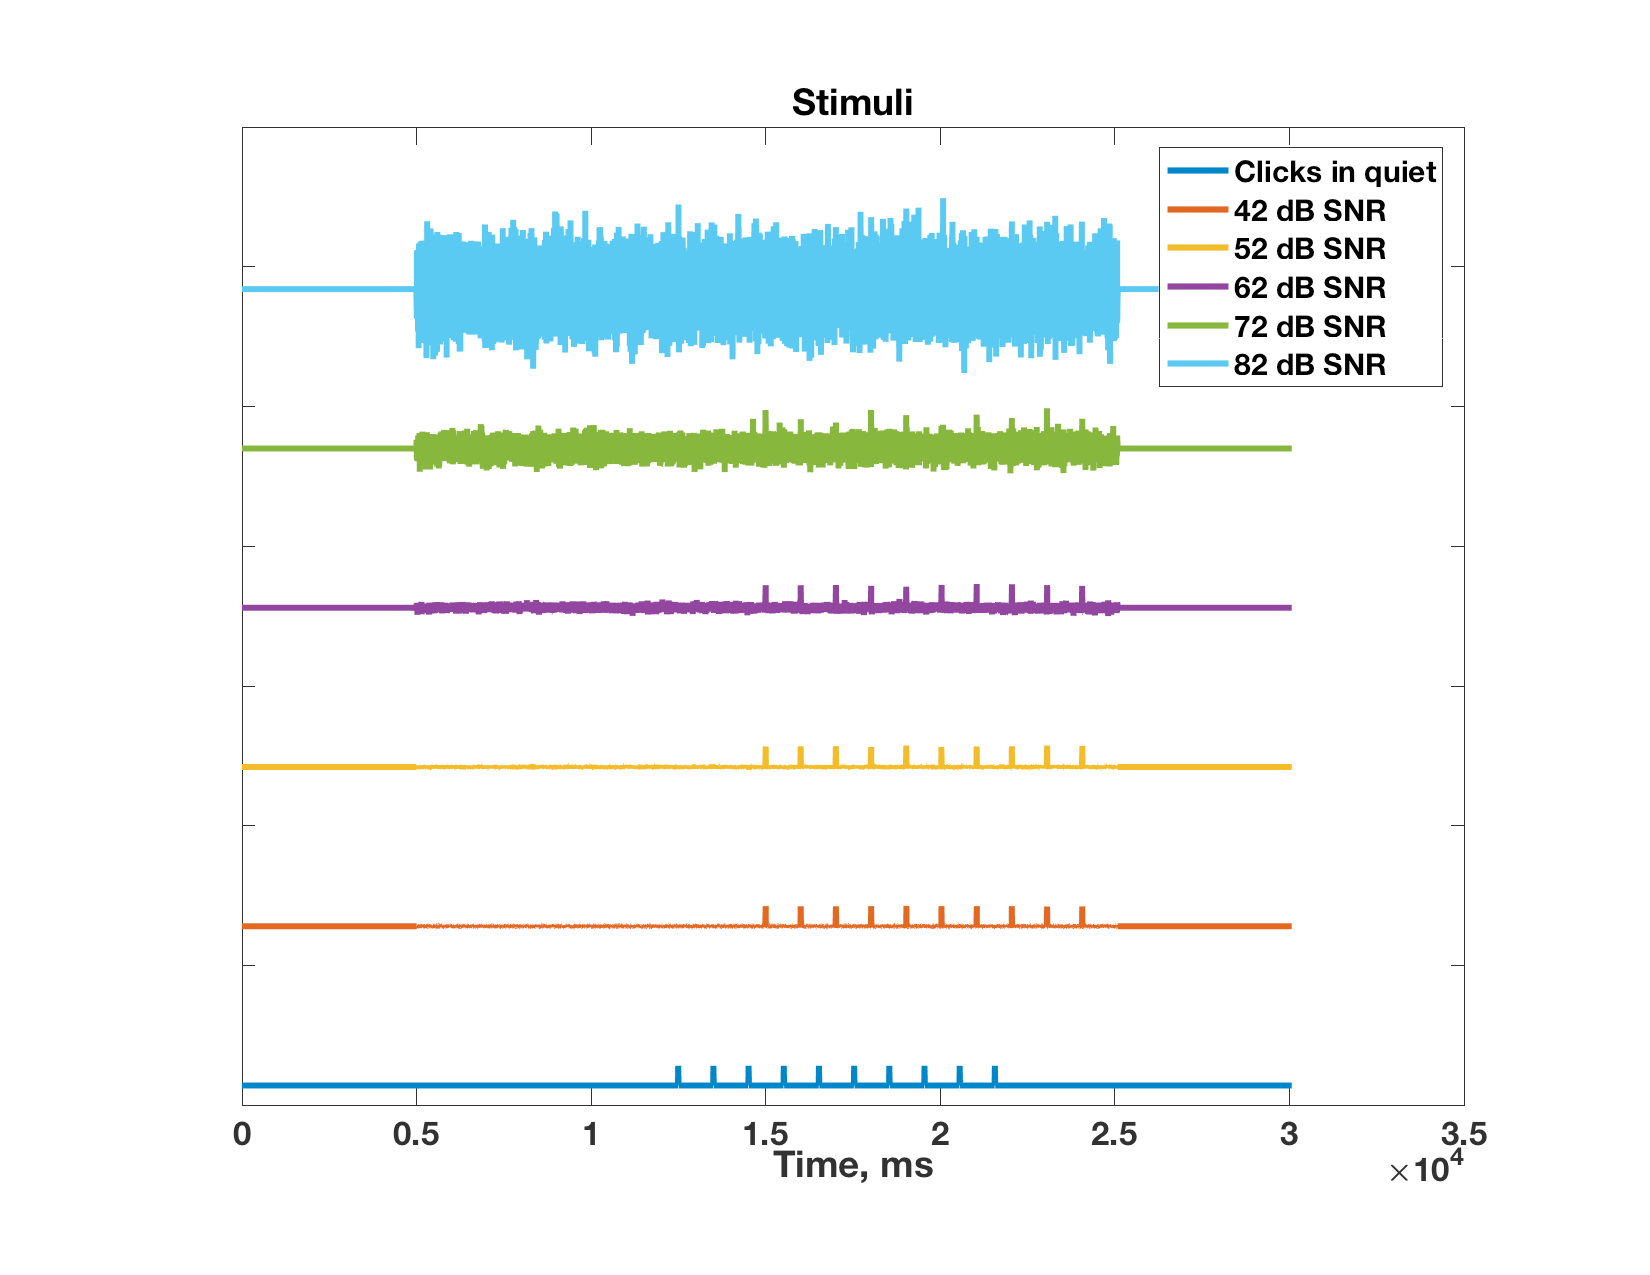
\includegraphics[width=\textwidth]{stimuli-used.pdf}
	\caption[Experimental Stimuli]{Stimuli used to drive the auditory models.  All stimuli were an 80dB SPL click train with a 100ms spacing between clicks.  A white Gaussian noise masker was added at five different masker levels.}
	\label{fig:stimuli-used}
\end{figure}

All other parameters values---choice of peripheral and brainstem model and logistically weighted fiber distributions---were fully explored.

In total, 240 separate simulations were run in parallel on Boston University's high-performance computing cluster over the course of approximately 9 days.  Model output was automatically stored into a HDF5 database approximately 250 GB in size.



\section{Effect of Cochlear Synaptopathy} % (fold)
\label{sec:effect_of_synaptopathy}
The effects of four types of synaptopathy---moderate, severe, low-SR specific moderate, and low-SR specific severe---were simulated, with the synaptic degradation parameters as given in \autoref{fig:synaptopathy}. 

\begin{figure}[htbp]
	\centering
	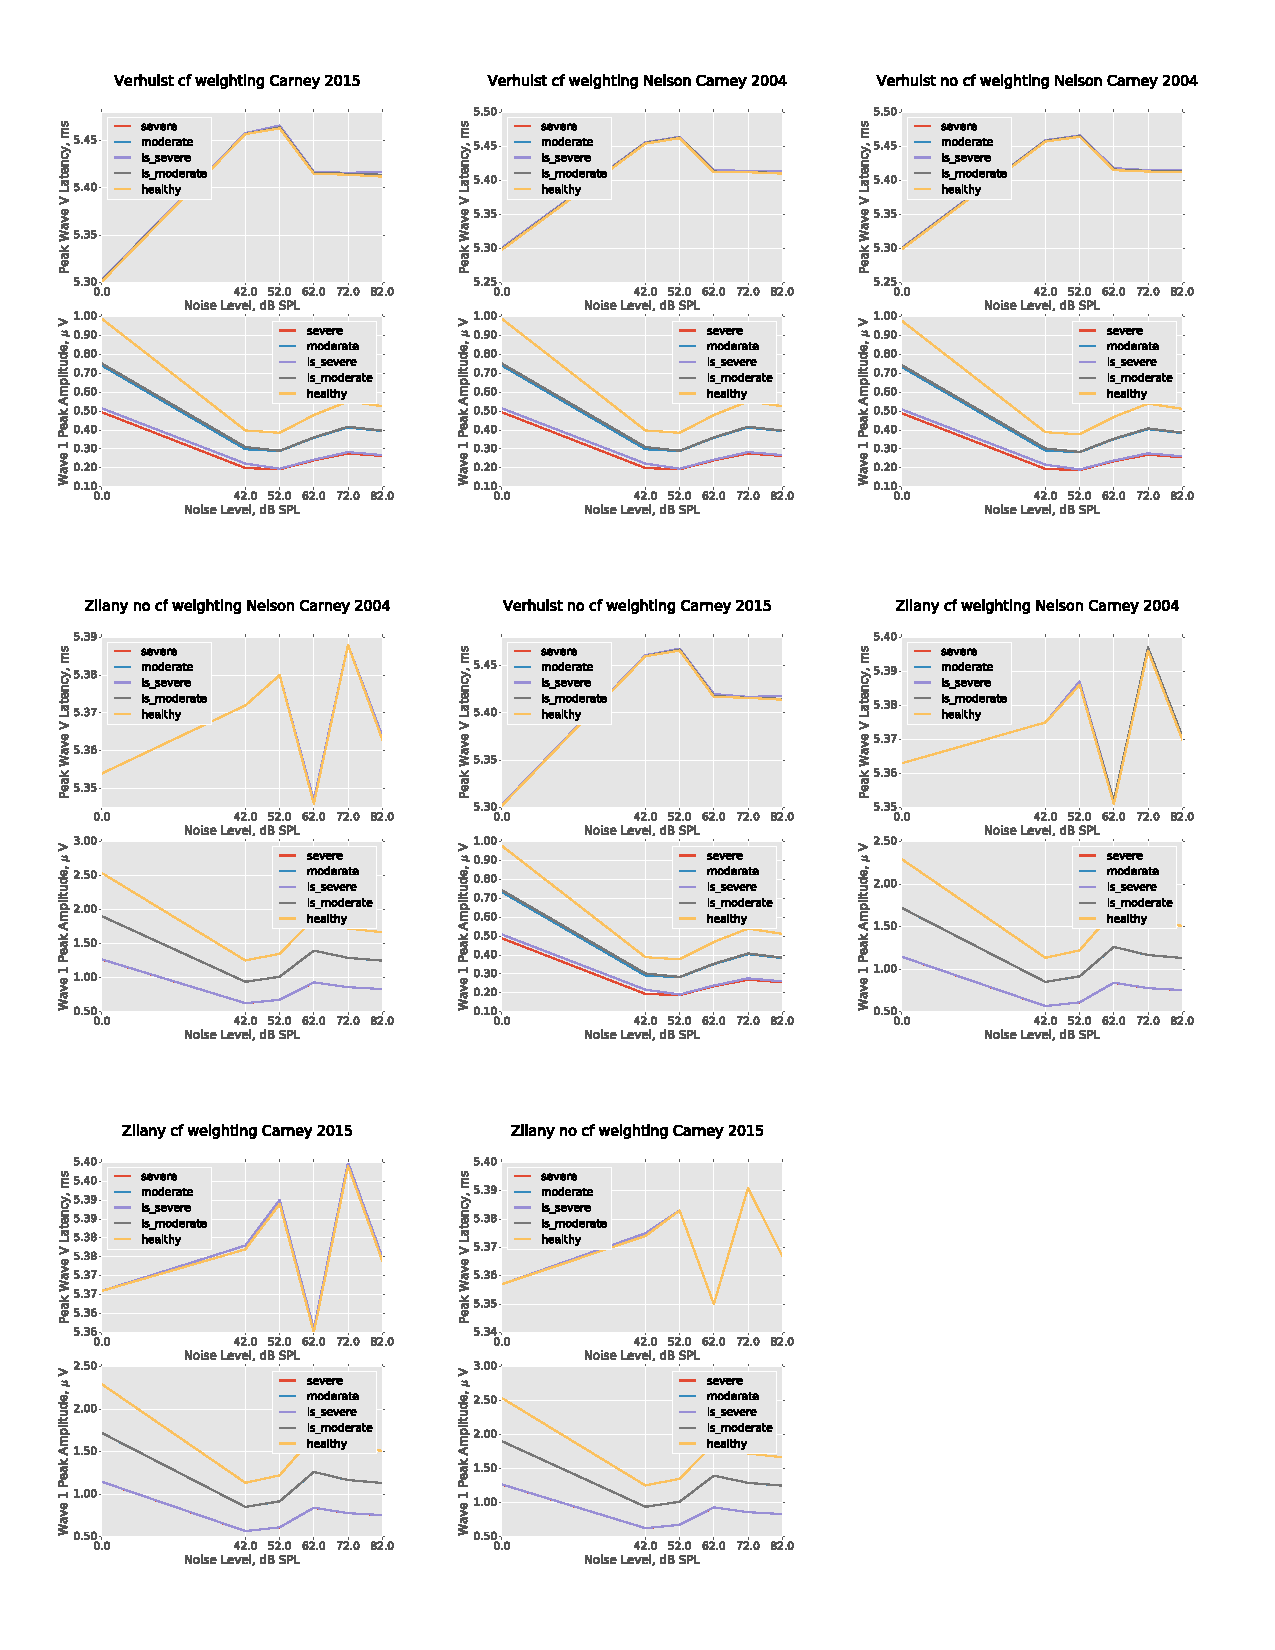
\includegraphics[width=\textwidth]{synaptopathy-all.pdf}
	\caption[Effects of Synaptopathy]{The effects of varying levels of synaptopathy on model responses to a stimulus at multiple noise levels.  Some traces are present but not visible as they precisely overlay other results.}
	\label{fig:synaptopathy_results}
\end{figure}

The effect of fiber loss on Wave V peak latency and Wave I peak amplitude for all other parameter combinations are given in \autoref{fig:synaptopathy_results}.  

Consistent with prediction and prior experiment, Wave I amplitudes decrease as a function of synaptopathy, as well as a function of increasing noise masker level.  Selective loss of low SR fibers closely follow their corresponding all-fiber degradation models, suggesting that low-SR degradation at the simulated severities don't contribute towards amplitude changes in the presence of high level noise maskers. 

Wave V latencies exhibit a consistent increase in latency relative to a pure click train,  consistent with observations by \citeauthor{Mehraei2016Auditory}, but latency magnitudes are not significantly affected by modeled synaptopathies. 
% section effect_of_synaptopathy (end)

\section{Effect of Peripheral Model Choice} % (fold)
\label{sec:effect_of_peripheral_model}
Because the response trends vary quite little as a function of the types of synaptopathy modeled in \autoref{sec:effect_of_synaptopathy}, the relative effects of model types can be explored while holding the type of synaptopathy fixed, thus eliminating one dimension of the parameter space.

The effects of peripheral model choice on Wave V peak latency and Wave I peak amplitudes are given in \autoref{fig:periphery_results}.   In general, the Verhulst model predicts both larger Wave V latencies and larger changes as a function of SNR compared to the Zilany model, which predicts generally small to no change in latencies.  This is contrary to earlier modeling results, which suggest the opposite effect of peripheral models. 

Wave I amplitude estimations follow similar shapes for each peripheral model.  While both produce physiologically plausible responses, the Verhulst model predicts amplitudes approximately half the magnitude of the Zilany model. 

\begin{figure}[htbp]
	\centering
	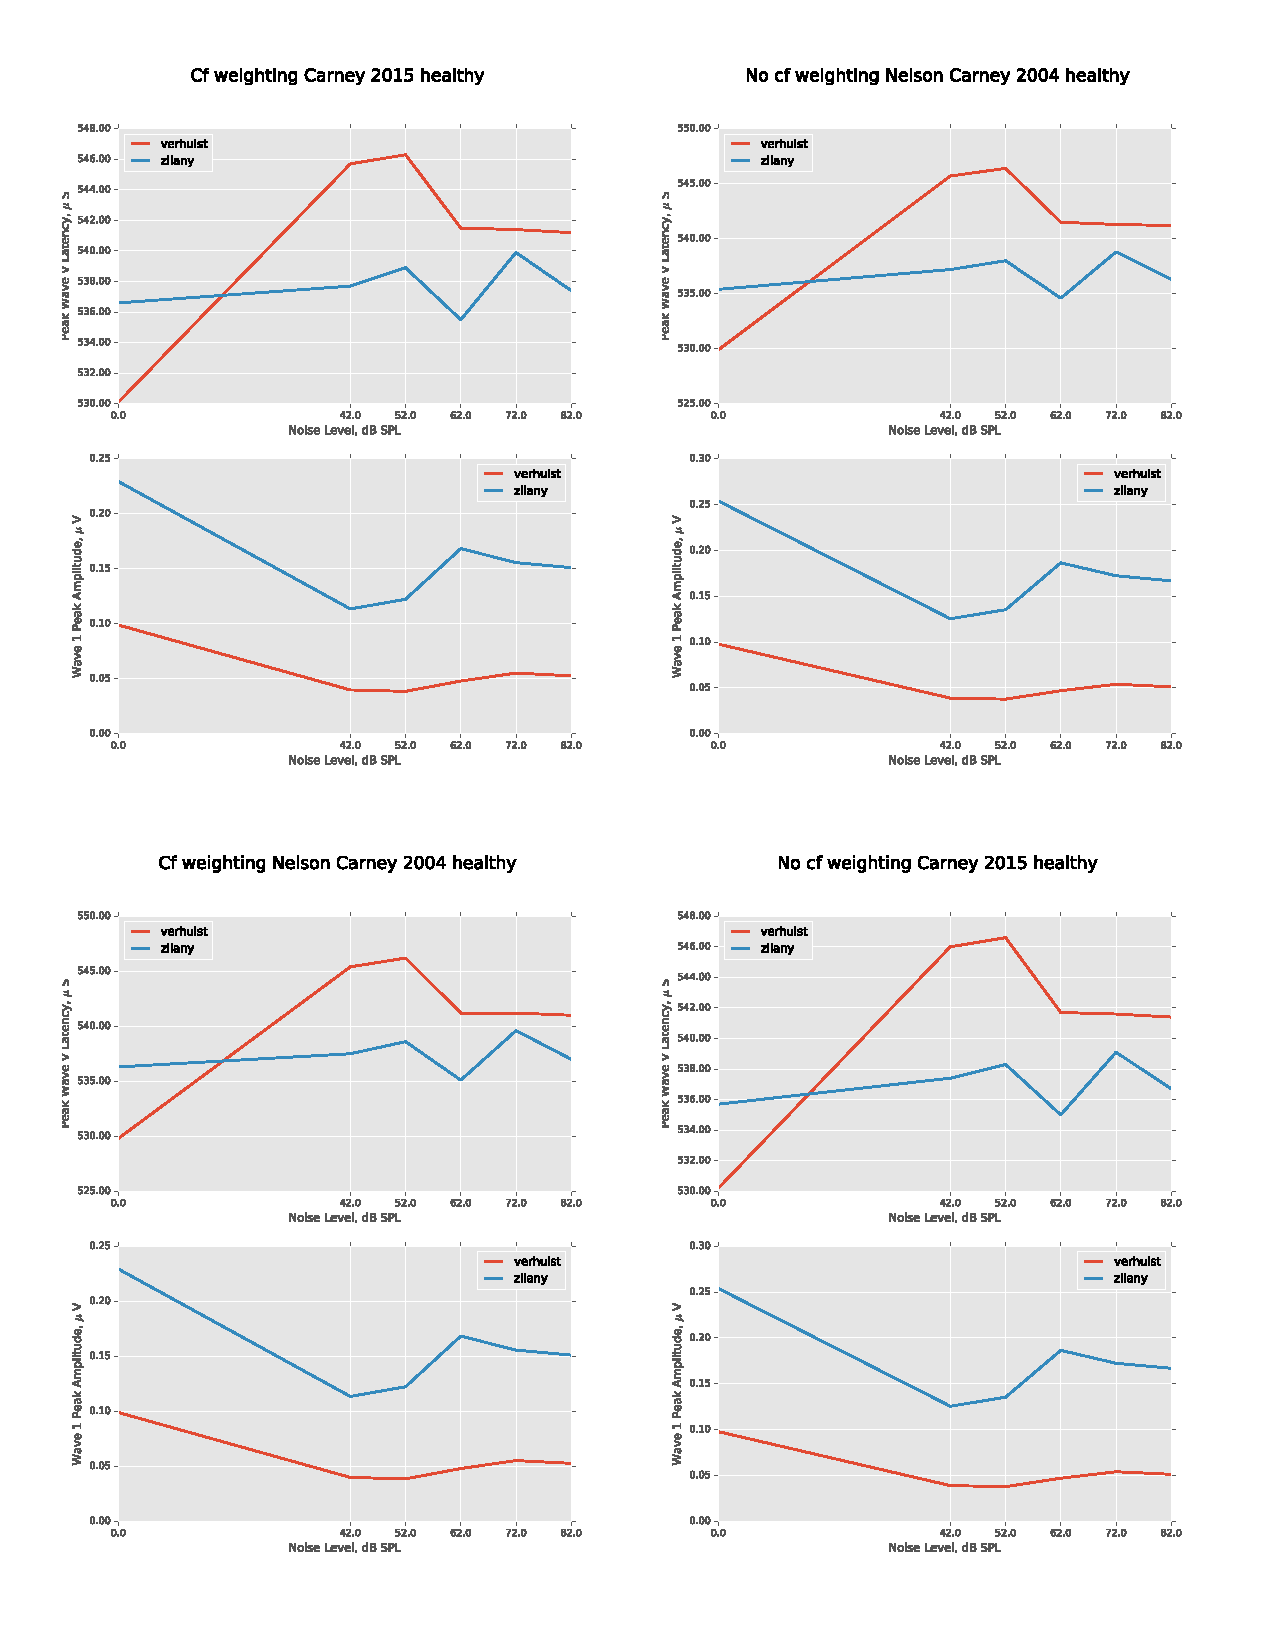
\includegraphics[width=\textwidth]{periphery-all.pdf}
	\caption[Effects of Peripheral Models]{Effects of Peripheral Models on Wave I peak amplitude and Wave V peak latency}
	\label{fig:periphery_results}
\end{figure}

% section effect_of_peripheral_model (end)


\section{Effect of CF weighting} % (fold)
\label{sec:effect_of_cf_weighting}
\begin{figure}[htbp]
	\centering
	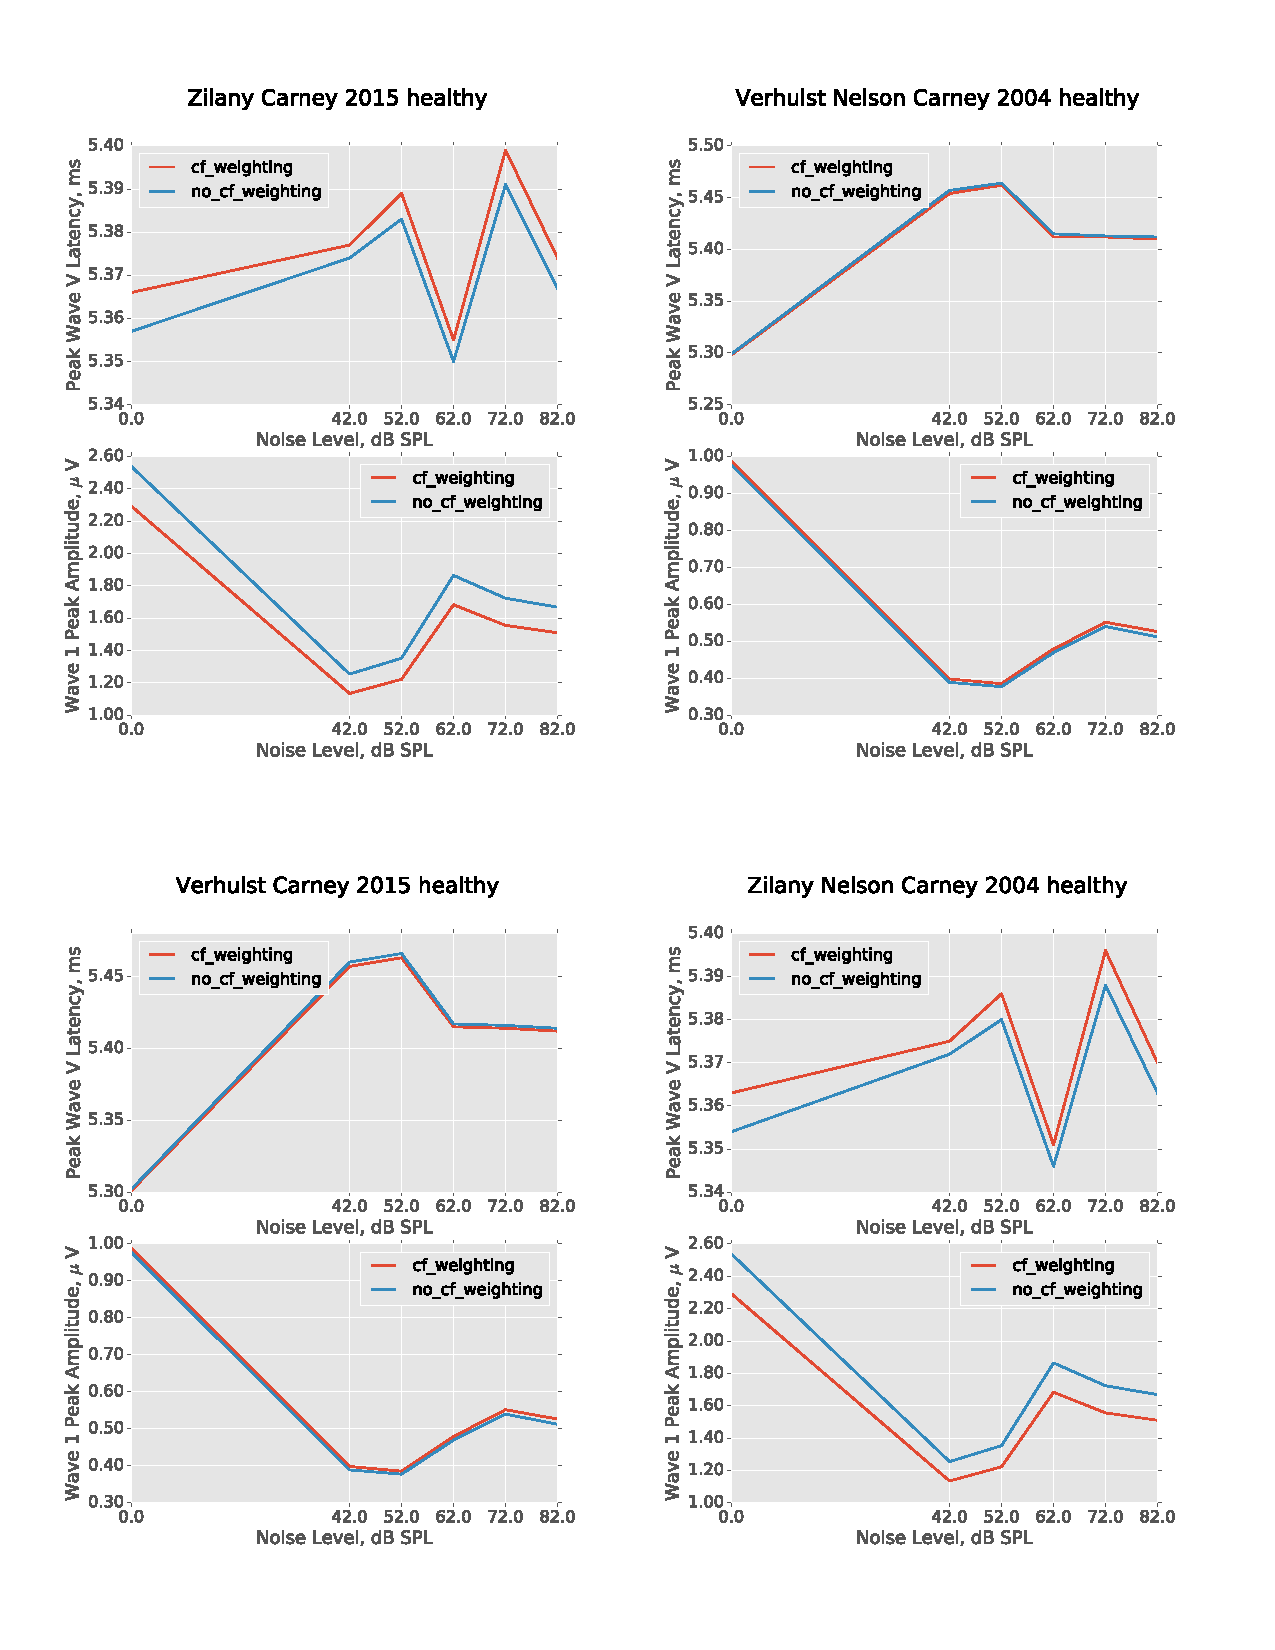
\includegraphics[width=\textwidth]{weighting-all.pdf}
	\caption[Effects of CF Weighting]{Effects of CF Weighting on Wave I peak amplitude and Wave V peak latency}
	\label{fig:cf_results}
\end{figure}

The effects of logistically weighing the fiber type distribution along the basilar membrane is given in \autoref{fig:cf_results}.  Surprisingly, there was very little relative effect with the Verhulst model to either Wave V latency or Wave I amplitude. 

In contrast, the Zilany model showed consistent suppression of Wave V latency and elevation of Wave I amplitudes relative to non-weighted responses.
% section effect_of_cf_weighting (end)

\section{Effect of Brainstem Model Choice} % (fold)
\label{sec:effect_of_brainstem_model}
\begin{figure}[htbp]
	\centering
	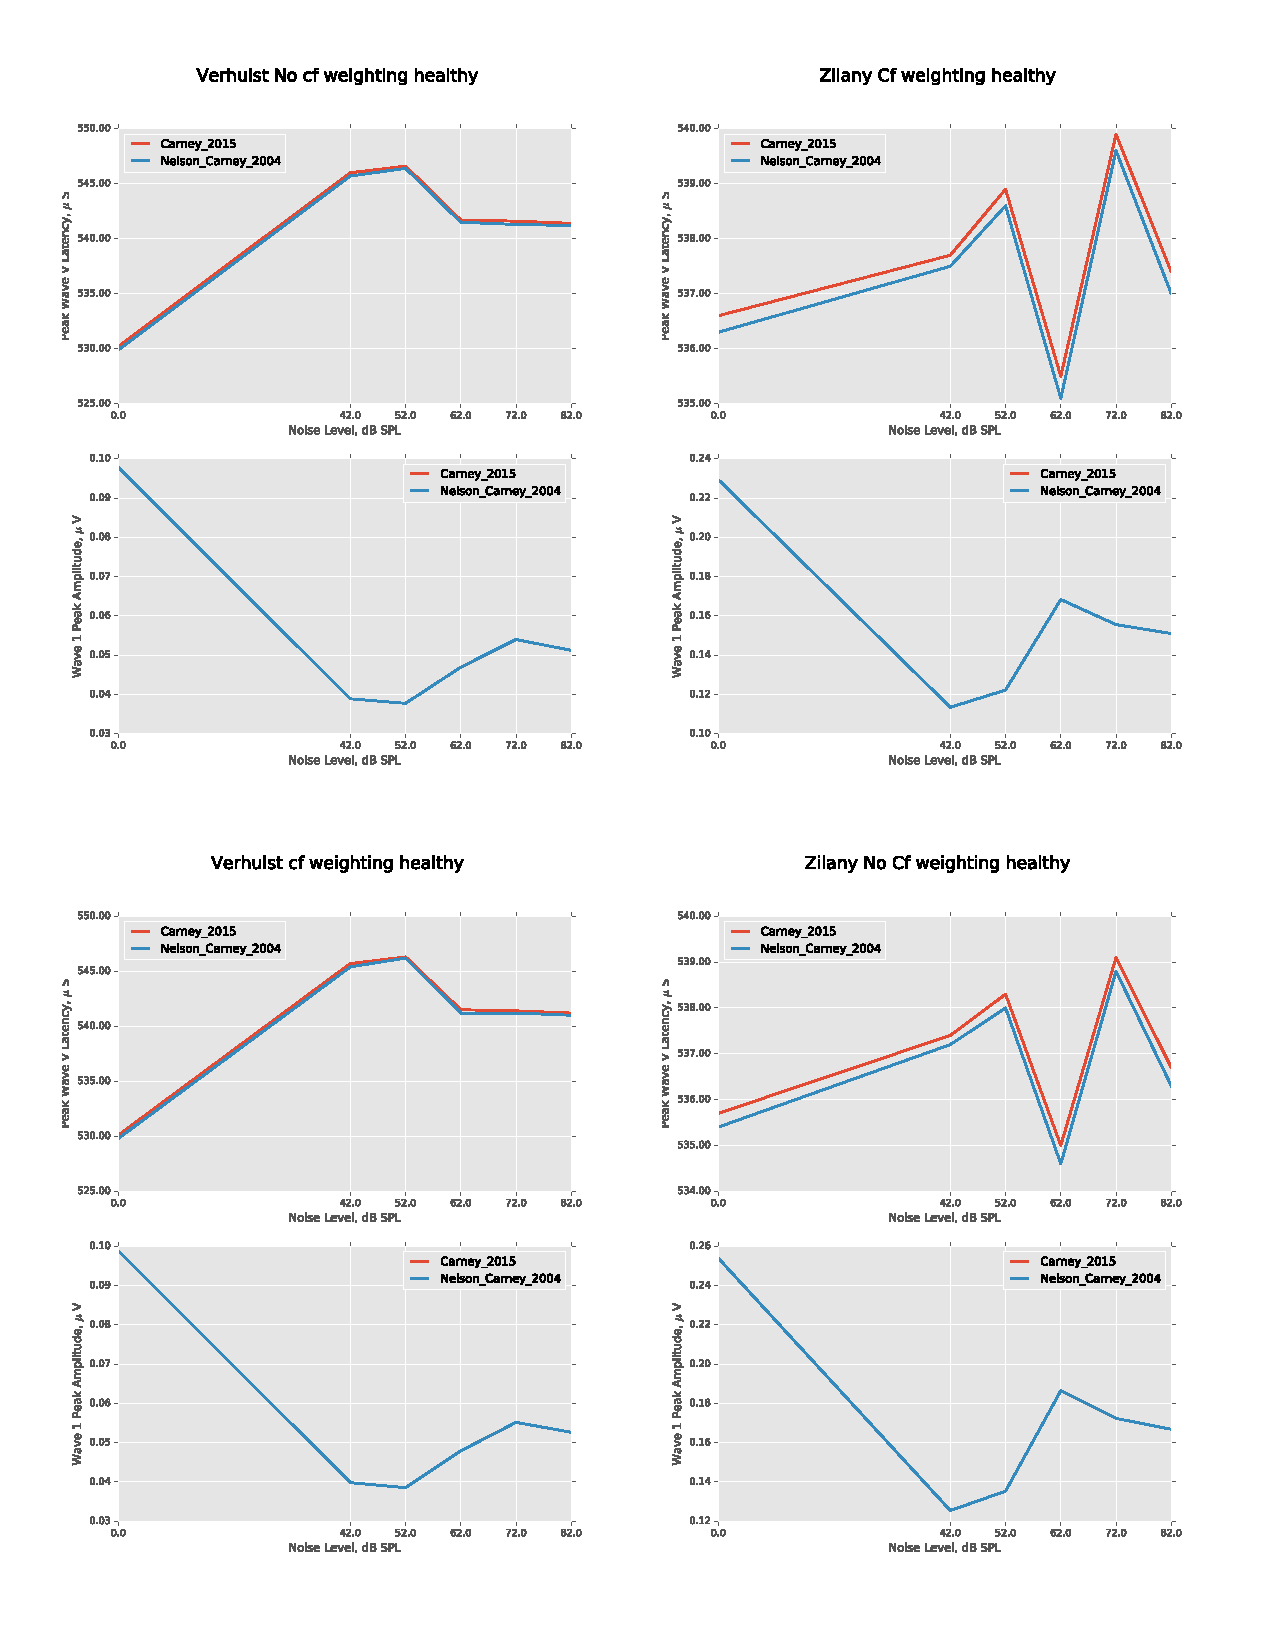
\includegraphics[width=\textwidth]{brainstem-all.pdf}
	\caption[Effects of Brainstem Models]{Effects of Brainstem Models on Wave V peak latencies.  Wave 1 amplitudes arise from the compound action potential of the AN alone, and are unaffected by the brainstem model.}
	\label{fig:brainstem_results}
\end{figure}

The effects of a more complex brainstem model is given in \autoref{fig:brainstem_results}.  No effects are observed for Wave I amplitudes, as Wave I originates at the level of the auditory nerve.  

Slight elevations of Wave V latencies are observed with the Zilany periphery. 
% section effect_of_brainstem_model (end)